\subsection{Leiterplatte}
In dieser Anwendung ist die Leiterplatte ein Raspberry Shield. Ein Shield sorgt dafür das alle Komponenten, die angesteuert werden sollen, übersichtlich an den \raspi angeschlossen werden. Es kann aber auch sein, dass das Shield eine Erweiterung für den \raspi ist.
In diesem Fall wurde das Shield verwendet, um die Komponenten mit dem \raspi zu verbinden.\\
\vspace{3mm}
PCB und der Schaltplan wurden in Eagle 7.0.0 entworfen.
\subsubsection{Schaltplan}
Das Shield wird über den PRT-14017\autocite{PRT-14017} Header mit dem \raspi verbunden\\
\vspace{3mm}
\begin{figure}[H]
\centering
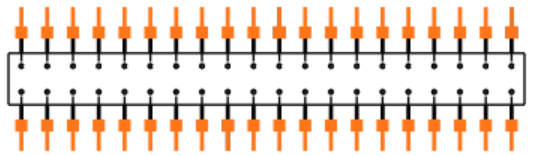
\includegraphics[scale=0.7]{image/prt140117.png}
\caption{Schaltplansymbol PRT-14017}
\end{figure}
Um die verschiedenen Komponenten anzuschließen, werden Schraubklemmen verwendet. Es werden fünf 4-Polige Schraubklemmen\autocite{4-polige-Schraubklemme} und elf 3-Polige Schraubklemmen\autocite{W237-103} benötigt.\\
\vspace{3mm}
Nachdem die Schraubklemmen und der Header platziert wurden, werden die Pole der Schraubklemmen mit dem Header verbunden. Die Zuordnung ist in der Tabelle 7 zu sehen. \\
\vspace{3mm}
\begin{table}[h]
    \centering
    \begin{tabular}{ | c | c | c | c | } 
  \hline
  \textbf{ Bezeichnung} & \textbf{ GPIO-Pin} & \textbf{ GPIO-Pin} & \textbf{ Versorgung}\\
  \hline
   Lüfter & GPIO19 & - & -  \\ 
  \hline
    Kühlung & GPIO12 & - & 5V  \\ 
  \hline
   LED-Streifen & GPIO20 & GPIO21 & - \\ 
  \hline
   Schlüsselschalter & GPIO06 & - & 3.3V \\ 
  \hline
   Ventil2 & GPIO25 & - & 5V \\
  \hline
   Notaus & GPIO05 & - & 3.3V \\
  \hline
   Ventil1 & GPIO24 & - & 5V \\
  \hline
   UV-Lampe & GPIO18 & GPIO23 & 5V \\
  \hline
   Endschalter & GPIO27 & GPIO22 & 5V \\
  \hline
   Motor & GPIO17 & GPIO13 PWM & - \\
  \hline
   Netzteil & GPIO14 & GPIO15 & 5V \\
  \hline
   Temperatursensor1 & GPIO07 & - & 5V \\
  \hline
   Temperatursensor2 & GPIO08 & - & 5V \\
  \hline
   Magnetsensor & GPIO16 & - & 3.3V \\
  \hline
   Drucksensor & GPIO03 SDA & GPIO05 SCL & 5V \\
  \hline
   UV-Sensor & GPIO03 SDA & GPIO05 SCL & 5V \\
  \hline
\end{tabular}
    \caption{Pinbelegung \raspi Shield}
\end{table}
\newpage
Der Drucksensor und der UV-Sensor sind beide über die I2C-Schnittstelle mit dem Raspberry Shield verbunden.\\
\vspace{3mm}
Information über die I2C-Schnittstelle sind unter \url{https://www.ti.com/lit/an/slva704/slva704.pdf?ts=1712280198725&ref_url=https%253A%252F%252Fwww.google.com%252F} zu finden.\\

\newpage
\begin{figure}[h]
\centering
    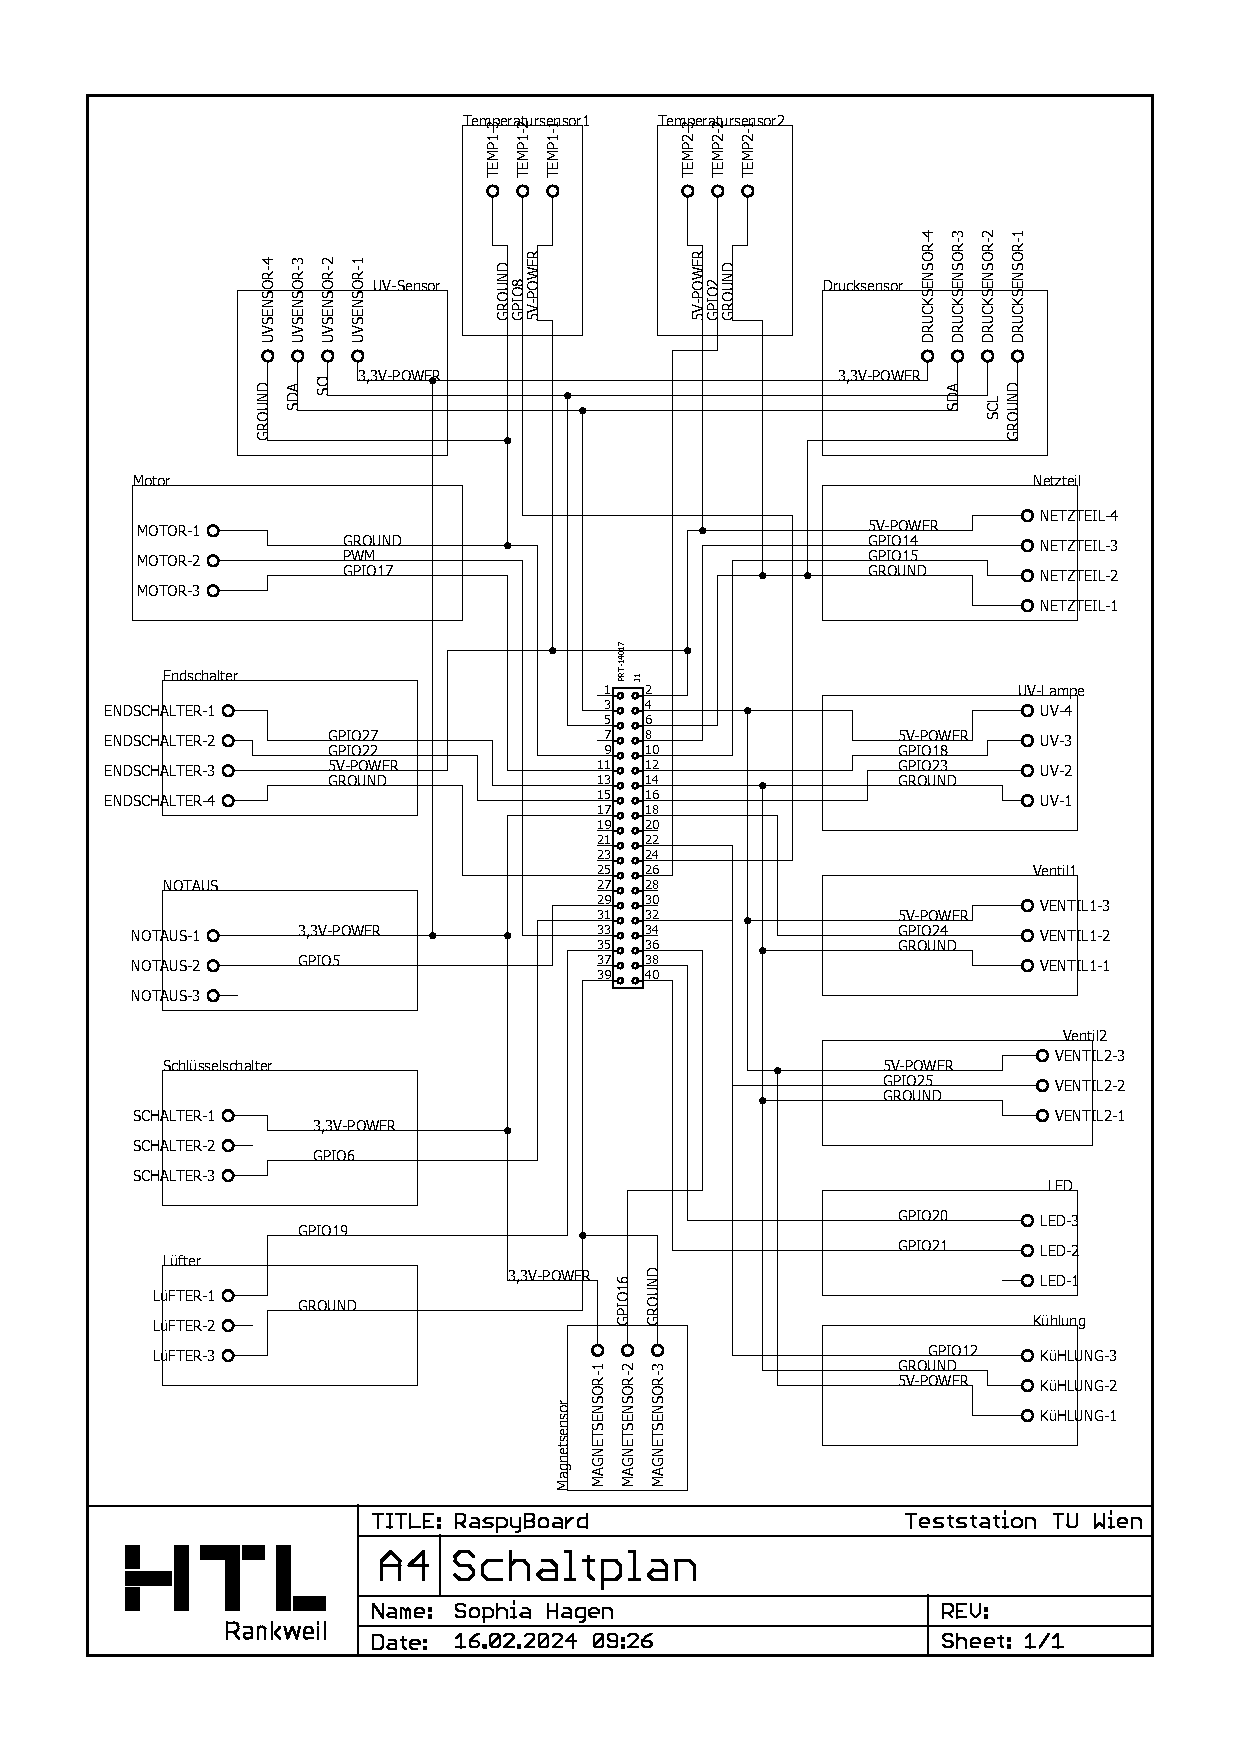
\includepdf[pages=1]{pdf/RaspyBoard_Schematic}
    %\caption{Schaltplan}
\end{figure}
\pagebreak
\subsubsection{PCB}
Die Platine hat eine Größe von \textit{95mm X 65mm}. Geplant war, das Board in der Größe des \raspi zu entwerfen. Der \raspi 4B besitzt 2 USB-Buchsen und und ein LAN-Anschluss. Diese sind jedoch zu hoch, um darüber eine Platine zu platzieren die mit dem \raspi verbunden werden soll. Aus diesem Grund wurde das Board in die Länge gezogen. Die 16 Schraubklemmen werden einzeln beschriftet. Beispielsweise hat die Schraubklemme für den UV-Sensor die Beschriftung UV-Sensor. Zur Befestigung werden 4 Bohrungen benötigt. Diese haben einen Durchmesser von \textit{3.5mm}.\\
\vspace{3mm}
\begin{figure}[H]
	\centering
	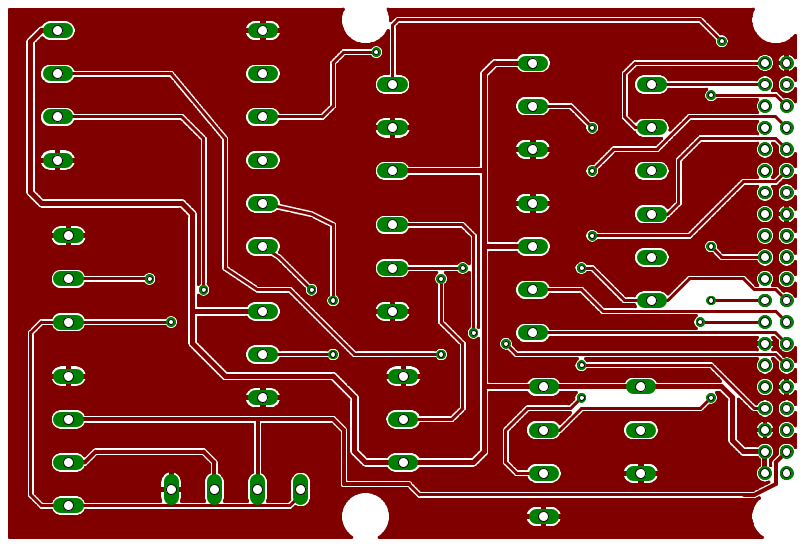
\includegraphics[scale=0.8]{image/layouttop.png}
	\caption{Layout Top}
	\label{fig:enter-label}
\end{figure}
\begin{figure}[H]
	\centering
	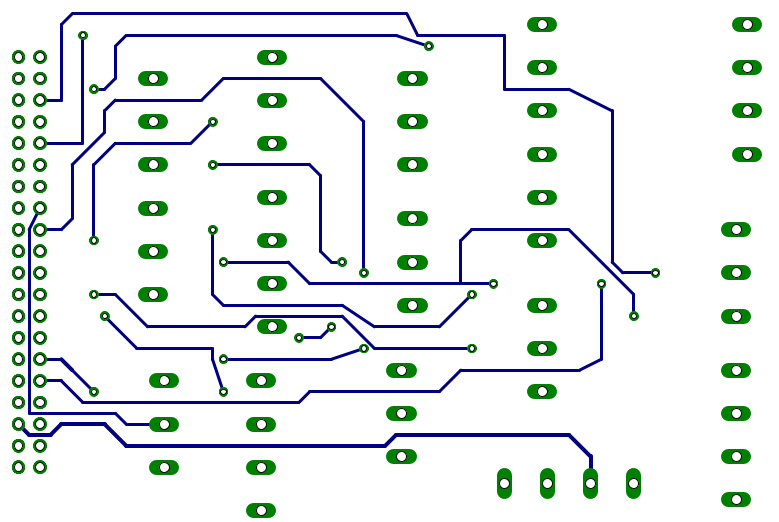
\includegraphics[scale=0.8]{image/layoutbottom.png}
	\caption{Layout Bottom}
	\label{fig:enter-label}
\end{figure}
\newpage
\begin{figure}[H]
	\centering
	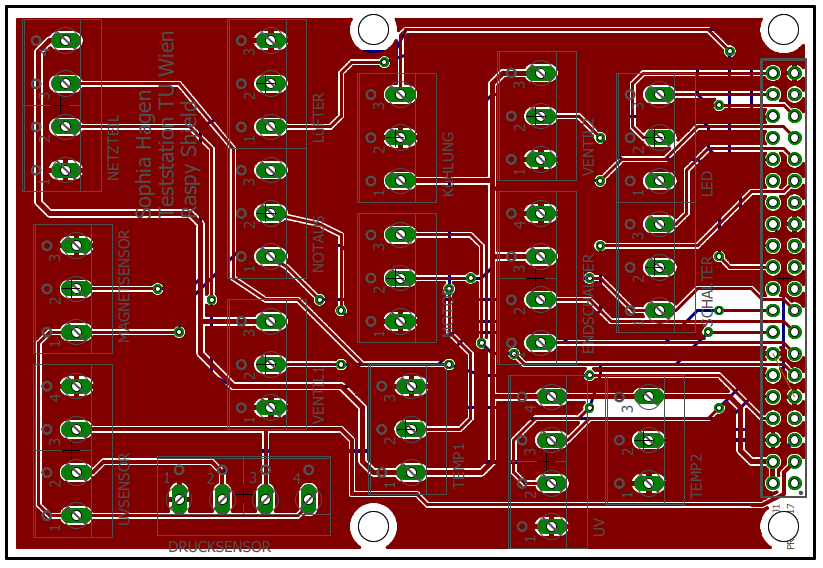
\includegraphics[scale=0.8]{image/workp.png}
	\caption{PCB mit Polygon}
	\label{fig:enter-label}
\end{figure}
\begin{figure}[H]
	\centering
	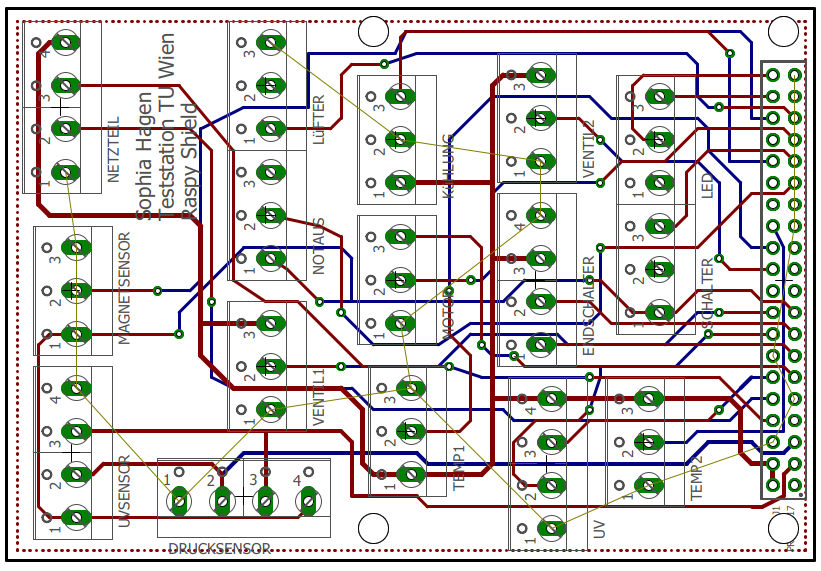
\includegraphics[scale=0.8]{image/worko.png}
	\caption{PCB ohne Polygon}
	\label{fig:enter-label}
\end{figure}
\pagebreak
\begin{figure}[H]
\centering
    \includegraphics[scale=0.27]{image/Platine_unbestückt.jpg}
    \caption{Unbestückte Platine}
\end{figure}
\begin{figure}[H]
\centering
    \includegraphics[scale=0.18]{image/platine_bestückt.jpg}
    \caption{Bestückte Platine}
\end{figure}